% LuaLaTeX

\documentclass[a4paper, twoside, 12pt]{article}
\usepackage[latin]{babel}
%\usepackage[landscape, left=3cm, right=1.5cm, top=2cm, bottom=1cm]{geometry} % okraje stranky
%\usepackage[landscape, a4paper, mag=1166, truedimen, left=2cm, right=1.5cm, top=1.6cm, bottom=0.95cm]{geometry} % okraje stranky
\usepackage[landscape, a4paper, mag=1400, truedimen, left=0.5cm, right=0.5cm, top=0.5cm, bottom=0.5cm]{geometry} % okraje stranky

\usepackage{fontspec}
\setmainfont[FeatureFile={junicode.fea}, Ligatures={Common, TeX}, RawFeature=+fixi]{Junicode}
%\setmainfont{Junicode}

% shortcut for Junicode without ligatures (for the Czech texts)
\newfontfamily\nlfont[FeatureFile={junicode.fea}, Ligatures={Common, TeX}, RawFeature=+fixi]{Junicode}

\usepackage{multicol}
\usepackage{color}
\usepackage{lettrine}
\usepackage{fancyhdr}

% usual packages loading:
\usepackage{luatextra}
\usepackage{graphicx} % support the \includegraphics command and options
\usepackage{gregoriotex} % for gregorio score inclusion
\usepackage{gregoriosyms}
\usepackage{wrapfig} % figures wrapped by the text
\usepackage{parcolumns}
\usepackage[contents={},opacity=1,scale=1,color=black]{background}
\usepackage{tikzpagenodes}
\usepackage{calc}
\usepackage{longtable}
\usetikzlibrary{calc}

\setlength{\headheight}{14.5pt}

% Commands used to produce a typical "Conventus" booklet

\newenvironment{titulusOfficii}{\begin{center}}{\end{center}}
\newcommand{\dies}[1]{#1

}
\newcommand{\nomenFesti}[1]{\textbf{\Large #1}

}
\newcommand{\celebratio}[1]{#1

}

\newcommand{\hora}[1]{%
\vspace{0.5cm}{\large \textbf{#1}}

\fancyhead[LE]{\thepage\ / #1}
\fancyhead[RO]{#1 / \thepage}
\addcontentsline{toc}{subsection}{#1}
}

% larger unit than a hora
\newcommand{\divisio}[1]{%
\begin{center}
{\Large \textsc{#1}}
\end{center}
\fancyhead[CO,CE]{#1}
\addcontentsline{toc}{section}{#1}
}

% a part of a hora, larger than pars
\newcommand{\subhora}[1]{
\begin{center}
{\large \textit{#1}}
\end{center}
%\fancyhead[CO,CE]{#1}
\addcontentsline{toc}{subsubsection}{#1}
}

% rubricated inline text
\newcommand{\rubricatum}[1]{\textit{#1}}

% standalone rubric
\newcommand{\rubrica}[1]{\vspace{3mm}\rubricatum{#1}}

\newcommand{\notitia}[1]{\textcolor{red}{#1}}

\newcommand{\scriptura}[1]{\hfill \small\textit{#1}}

\newcommand{\translatioCantus}[1]{\vspace{1mm}%
{\noindent\footnotesize \nlfont{#1}}}

% pruznejsi varianta nasledujiciho - umoznuje nastavit sirku sloupce
% s prekladem
\newcommand{\psalmusEtTranslatioB}[3]{
  \vspace{0.5cm}
  \begin{parcolumns}[colwidths={2=#3}, nofirstindent=true]{2}
    \colchunk{
      \input{#1}
    }

    \colchunk{
      \vspace{-0.5cm}
      {\footnotesize \nlfont
        \input{#2}
      }
    }
  \end{parcolumns}
}

\newcommand{\psalmusEtTranslatio}[2]{
  \psalmusEtTranslatioB{#1}{#2}{8.5cm}
}


\newcommand{\canticumMagnificatEtTranslatio}[1]{
  \psalmusEtTranslatioB{#1}{temporalia/extra-adventum-vespers/magnificat-boh.tex}{12cm}
}
\newcommand{\canticumBenedictusEtTranslatio}[1]{
  \psalmusEtTranslatioB{#1}{temporalia/extra-adventum-laudes/benedictus-boh.tex}{10.5cm}
}

% volne misto nad antifonami, kam si zpevaci dokresli neumy
\newcommand{\hicSuntNeumae}{\vspace{0.5cm}}

% prepinani mista mezi notovymi osnovami: pro neumovane a neneumovane zpevy
\newcommand{\cantusCumNeumis}{
  \setgrefactor{17}
  \global\advance\grespaceabovelines by 5mm%
}
\newcommand{\cantusSineNeumas}{
  \setgrefactor{17}
  \global\advance\grespaceabovelines by -5mm%
}

% znaky k umisteni nad inicialu zpevu
\newcommand{\superInitialam}[1]{\gresetfirstlineaboveinitial{\small {\textbf{#1}}}{\small {\textbf{#1}}}}

% pars officii, i.e. "oratio", ...
\newcommand{\pars}[1]{\textbf{#1}}

\newenvironment{psalmus}{
  \setlength{\parindent}{0pt}
  \setlength{\parskip}{5pt}
}{
  \setlength{\parindent}{10pt}
  \setlength{\parskip}{10pt}
}

%%%% Prejmenovat na latinske:
\newcommand{\nadpisZalmu}[1]{
  \hspace{2cm}\textbf{#1}\vspace{2mm}%
  \nopagebreak%

}

% mode, score, translation
\newcommand{\antiphona}[3]{%
\hicSuntNeumae
\superInitialam{#1}
\includescore{#2}

#3
}
 % Often used macros
%%%% Preklady jednotlivych zpevu (nektere se opakuji, a je dobre mit je
% vsechny na jedne hromade)

\newcommand{\trOratioAnteOfficium}{\translatioCantus{Otevři, Pane, má ústa, abych chválil tvé svaté jméno.
Očisti mé srdce od všech marnivých, zvrácených a~jiných myšlenek, osvěť rozum, rozněť cit,
abych mohl důstojně, soustředěně a~zbožně recitovat a~vysloužil si být
vyslyšen před tváří tvé velebnosti. Skrze Krista…}}

\newcommand{\trOratioPostOfficium}{\translatioCantus{\textit{Následující modlitbu
opatřil pro ty, kdo ji zbožně vyřknou po hodinkách, zesnulý papež Lev X.
odpustky za hříchy vzniklé při konání hodinek z~lidské křehkosti. Říká se
vkleče.}
Svatosvaté a~nerozdílné Trojici, ukřižovanému lidství našeho Pána Ježíše
Krista, přeblažené a~přeslavné plodné neporušenosti vždy Panny Marie
i~souhrnu všech svatých buď ode všeho stvoření věčná chvála, čest a~sláva, nám
pak buď dáno odpuštění všech hříchů, po nekonečné věky věků. Amen.}}

% HOURS ---

\newcommand{\trAntI}{\translatioCantus{Jasné narození slavné Panny Marie,
z pokolení (dosl. ze semene) Abrahámova, vzešlé z kmene Judova, z rodu Davidova.}}
\newcommand{\trAntII}{\translatioCantus{Dnes je Narození svaté Panny 
Marie, jejíž předrahý život osvěcuje všechny církve.}}

\newcommand{\trAntIII}{\translatioCantus{Maria, jež vzešla 
z královského rodu, září; myslí i duchem ji zbožně prosíme, aby 
nám pomáhala svými přímluvami.}}

\newcommand{\trAntIV}{\translatioCantus{Srdcem i duchem pějme Kristu 
k slávě o této svaté slavnosti vznešené Rodičky Boží Marie.}}

\newcommand{\trAntV}{\translatioCantus{Příjemně \notitia{?} 
oslavujme Narození blahoslavené Marie,
aby se ona za nás přimlouvala u Pána Ježíše Krista.}}

\newcommand{\trCapituli}{\translatioCantus{Před věky, na počátku mě stvořil, potrvám věčně. Ve svatém Stanu jsem před ním konala službu.}}

\newcommand{\trRespVesp}{\translatioCantus{Buď zdráva, Maria,
plná milosti: \grestar{} Pán s tebou. \Vbardot{} Požehnaná jsi mezi ženami,
a požehnaný plod života (ve smyslu lůna, břicha) tvého.}}

\newcommand{\trVersus}{\translatioCantus{\Vbardot{} Dnes je Narození svaté Panny Marie. \Rbardot{} Jejíž předrahý život osvěcuje všechny církve.}}

\newcommand{\trAntMagnificatI}{\translatioCantus{Konejme památku
veledůstojného narození slavné Panny Marie,
jíž se dostalo mateřské důstojnosti bez ztráty panenské cudnosti.}}

% Tento preklad je vice nez nejisty a ani alternativy, ktere jsem
% videl, me nepresvedcily...
\newcommand{\trAntBenedictus}{\translatioCantus{Slavnostně slavme 
dnešní narození Marie, vždy Panny a Rodičky Boží: v něm se objevuje
vysokost trůnu (totiž Marie, trůnu Božího Syna), aleluja.}}

\newcommand{\trAntMagnificatII}{\translatioCantus{Tvé narození,
Bohorodičko Panno, vyhlásilo radost celému světu:
z tebe totiž vzešlo Slunce spravedlnosti, Kristus, náš Bůh:
jenž zrušil kletbu a dal nám požehnání: přemohl smrt a dal nám život věčný.}}

\newcommand{\trOrationis}{\translatioCantus{Prosíme tě, Bože, 
uděl svým služebníkům dar nebeské milosti,
aby těm, jimž slehnutím blahoslavené Panny vyvstal počátek spásy, 
slavnost k poctě jejího narození přinesla
rozhojnění pokoje.
Skrze tvého Syna, našeho Pána Ježíše Krista, který s tebou žije a kraluje,
Bůh, v jednotě Ducha svatého po všechny věky věků.}}

\newcommand{\trFideliumAnimae}{\translatioCantus{\Vbardot{} Duše věrných ať pro
milosrdenství Boží odpočívají v~pokoji. \Rbardot{} Amen.}}

% Completorium

\newcommand{\trJubeDomne}{\translatioCantus{Rač, pane, požehnat.}}

\newcommand{\trComplBenedictio}{\translatioCantus{Pokojnou noc a~svatou smrt
nechť nám dopřeje všemohoucí Pán. \Rbardot{} Amen.}}

\newcommand{\trComplLectioBr}{\translatioCantus{Buďte střízliví, bděte.
Váš protivník Ďábel obchází jako lev řvoucí a~hledá, koho by pohltil.
Postavte se proti němu pevní ve víře.  Ale ty, Pane, smiluj se nad námi.
\Rbardot{} Bohu díky.}}

\newcommand{\trComplAntI}{\translatioCantus{Rač se smilovati nade mnou,
Hospodine, a vyslyš mou modlitbu.}}

\newcommand{\trComplCapituli}{\translatioCantus{Jsi přece, Hospodine,
uprostřed nás a~jmenujeme se po tobě.  Neopouštěj nás, Pane, náš Bože.}}

\newcommand{\trRespCompl}{\translatioCantus{Do tvých rukou, Pane, \grestar{}
poroučím svého ducha. \Vbardot{} Ty mne zachráníš, Pane, Bože věrný.}}

\newcommand{\trComplVersus}{\translatioCantus{\Vbardot{} Střez mne jako zřítelnici oka,
aleluja. \Rbardot{} Ve stínu svých křídel uschovej mne, aleluja.}}

\newcommand{\trAntSalvaNos}{\translatioCantus{Ochraňuj nás, Pane, když
bdíme, a~buď s~námi, když spíme, ať bdíme s~Kristem a~odpočíváme v~pokoji.}}

\newcommand{\trComplOrationis}{\translatioCantus{Zavítej, prosíme, Pane, sem
do našeho příbytku a~daleko od něj zažeň všechny úklady nepřítele. Ať tu
bydlí tví svatí andělé a~tvoje požehnání buď nad ním stále. Skrze…}}

\newcommand{\trSalveRegina}{\translatioCantus{Zdrávas Královno, matko
milosrdenství, živote, sladkosti a naděje naše, buď zdráva!
K tobě voláme, vyhnaní synové Evy,
k tobě vzdycháme, lkajíce a plačíce
v tomto slzavém údolí.
A proto, orodovnice naše,
obrať k nám své milosrdné oči
a Ježíše, požehnaný plod života svého,
nám po tomto putování ukaž,
ó milostivá, ó přívětivá,
ó přesladká, Panno Maria!}}

\newcommand{\trOraProNobis}{\translatioCantus{\Vbardot{} 
Oroduj za nás, svatá Boží Rodičko,
\Rbardot{} aby nám Kristus dal účast na svých zaslíbeních.}}

% Matutinum

\newcommand{\trMatInvitatorium}{\translatioCantus{}}

\newcommand{\trMatVeniteA}{\translatioCantus{Pojďte, chvalme s~radostí Pána,
s~jásotem slavme Boha, svou spásu; předstupme před tvář jeho s~díky, písně plesu pějme jemu.}}

\newcommand{\trMatVeniteB}{\translatioCantus{Neboť Bůh veliký jest Hospodin, a~král nade všecky bohy.
Jsouť v~jeho ruce všecky hlubiny země, temena hor jsou majetek jeho.}}

\newcommand{\trMatVeniteC}{\translatioCantus{Jehoť jest moře, neb on je učinil; i~souš
je dílo jeho rukou. Pojďme, klanějme se, padněme, klekněme před Pánem, svým
tvůrcem. Jeť on Pán, náš Bůh, a~my jsme lid, jejž on vodí a~ovce, jež pase.}}

\newcommand{\trMatVeniteD}{\translatioCantus{Kéž byste poslechli dnes hlasu jeho:
,,Nezatvrzujte svých srdcí jak v~Hádce, jak v~Pokušení na poušti, kde vaši otcové pokoušeli mne,
zkoušeli mne, ač vídali skutky mé.``}}

\newcommand{\trMatVeniteE}{\translatioCantus{Čtyřicet roků mrzel jsem se na to pokolení
a~řekl jsem: ,,Lid je to myslí stále bloudící``! Oni však nechtěli znáti mé cesty, takže jsem
přisáhl ve svém hněvu: ,,Nedojdou odpočinku mého!\mbox{}``}}

\newcommand{\trMatAntI}{\translatioCantus{}}

\newcommand{\trMatAntII}{\translatioCantus{}}

\newcommand{\trMatAntIII}{\translatioCantus{}}

\newcommand{\trMatVersusI}{\translatioCantus{}}

\newcommand{\trMatAbsolutioI}{\translatioCantus{Vyslyš Pane Ježíši Kriste
prosby svých služebníků \gredagger{} a~smiluj se nad námi, \grestar{} jenž
s~Otcem a~Duchem…}}

\newcommand{\trMatBenedictioI}{\translatioCantus{Rač, pane, požehnat.
Věčný Otec nám stále žehnej. \Rbardot{} Amen.}}

\newcommand{\trMatLecI}{\translatioCantus{Kéž by mě zulíbal polibky svých úst. 
Tvé milování je nad víno lahodnější;
vybraně voní tvé voňavky;
rozlévající se olej je tvé jméno,
proto tě dívky milují.
Strhni mě za sebou, poběžme!
Král mě uvedl do svých komnat;
budeš nám radostí a jásotem.
Víc než víno oslavíme tvé milování;
věru po právu jsi milován!
Snědá jsem, a přece krásná, jeruzalémské dcery,
jako stany kedarské,
jako šalmské závěsy.
}}

\newcommand{\trMatRespI}{\translatioCantus{}}

\newcommand{\trMatBenedictioII}{\translatioCantus{Rač, pane, požehnat.
Jednorozený Boží Syn nám žehnej \grestar{} a nám pomáhej. \Rbardot{} Amen.}}

\newcommand{\trMatLecII}{\translatioCantus{Nehleďte na mou osmahlou pleť:
to mě slunce ožehlo.
Synové mé matky se na mne rozzlobili,
poslali mě hlídat vinice.
A svou vinici, tu jsem nehlídala!
Pověz mi tedy, ty, jehož miluje mé srdce:
kam zavedeš své stádo pást,
kde ho necháš za poledne odpočívat?
Abych už nebloudila jako tulačka
poblíž stád druhů tvých.
Nevíš-li to, nejrásnější z žen,
jdi po stopách stáda
a kůzlata svá zaveď, ať se pasou
poblíž obydlí pastýřů.
Ke své klisně zapřažené do vozu faraonova
tebe, mé milá, přirovnávám.
Stále krásné jsou tvé líce s náušnicemi
i tvé hrdlo v náhrdelnících.}}

\newcommand{\trMatRespII}{\translatioCantus{}}

\newcommand{\trMatBenedictioIII}{\translatioCantus{Rač, pane, požehnat.
Milost Ducha Svatého ať osvítí nám smysly \grestar{} i srdce. \Rbardot{} Amen.}}

\newcommand{\trMatLecIII}{\translatioCantus{Zhotovíme ti zlaté náušnice
a kuličky ze stříbra.
Když král stoluje,
vydechuje můj nard svou vůni.
Můj milý je polštářek s myrhou,
jenž mi odpočívá mezi ňadry.
Můj milý je hrozen šáchoru
ve vinicích v Engadi.
Jak jsi krásná, milá moje,
jak jsi krásná!
Tvé oči jsou holubice.
Jak jsi krásný, můj milý,
jak líbezný!
Naše lože je samá zeleň.
Trámoví našeho domu je z cedru,
naše ostění z cypřiše.}}

\newcommand{\trMatRespIII}{\translatioCantus{}}

\newcommand{\trMatAntIV}{\translatioCantus{}}

\newcommand{\trMatAntV}{\translatioCantus{}}

\newcommand{\trMatAntVI}{\translatioCantus{}}

\newcommand{\trMatVersusII}{\translatioCantus{}}

\newcommand{\trMatAbsolutioII}{\translatioCantus{
Tvá milost a laskavost nechť nám pomáhá, jenž žiješ a vládneš s Otcem a Svatým Duchem na věky věků.}}

\newcommand{\trMatBenedictioIV}{\translatioCantus{Rač, pane, požehnat.
Bůh Otec všemohoucí, \grestar{} buď k nám milostivý a odpouštějící. \Rbardot{} Amen.}}

\newcommand{\trMatLecIV}{\translatioCantus{}}

\newcommand{\trMatRespIV}{\translatioCantus{}}

\newcommand{\trMatBenedictioV}{\translatioCantus{}}

\newcommand{\trMatLecV}{\translatioCantus{}}

\newcommand{\trMatRespV}{\translatioCantus{}}

\newcommand{\trMatBenedictioVI}{\translatioCantus{Rač, pane, požehnat.
Bůh rozněť v nás oheň své lásky. \Rbardot{} Amen.}}

\newcommand{\trMatLecVI}{\translatioCantus{}}

\newcommand{\trMatRespVI}{\translatioCantus{}}

\newcommand{\trMatAntVII}{\translatioCantus{}}

\newcommand{\trMatAntVIII}{\translatioCantus{}}

\newcommand{\trMatAntIX}{\translatioCantus{}}

\newcommand{\trMatVersusIII}{\translatioCantus{}}

\newcommand{\trMatAbsolutioIII}{\translatioCantus{Z okovů našich hříchů,
\grestar{} vysvoboď nás všemohoucí a milosrdný Pán. \Rbardot{} Amen.}}

\newcommand{\trMatBenedictioVII}{\translatioCantus{Rač, pane, požehnat.
Čtení evangelia nechť je nám \grestar{} spásou a ochranou. \Rbardot{} Amen.}}

\newcommand{\trMatLecVIIa}{\translatioCantus{
  Rodokmen Ježíše Krista, syna Davidova, syna Abrahámova:
  Abrahám zplodil Izáka,
  Izák zplodil Jakuba.}}

\newcommand{\trMatLecVIIb}{\translatioCantus{}}

\newcommand{\trMatRespVII}{\translatioCantus{}}

\newcommand{\trMatBenedictioVIII}{\translatioCantus{Rač, pane, požehnat.
\Rbardot{} Amen.}}

\newcommand{\trMatLecVIII}{\translatioCantus{}}

\newcommand{\trMatRespVIII}{\translatioCantus{}}

\newcommand{\trMatBenedictioIX}{\translatioCantus{Rač, pane, požehnat.
Do společnosti občanů nebes \grestar{} ať nás dovede král andělů.
\Rbardot{} Amen.}}

\newcommand{\trMatLecIX}{\translatioCantus{}}

% from the Czech Liturgia horarum
\newcommand{\trTeDeum}{\begin{translatioMulticol}{3}

Bože, tebe chválíme, 
tebe, Pane, velebíme.

Tebe, věčný Otče, 
oslavuje celá země.

Všichni andělé, 
cherubové i~serafové,

všechny mocné nebeské zástupy 
bez ustání volají:

Svatý, Svatý, Svatý, 
Pán, Bůh zástupů.

Plná jsou nebesa i~země 
tvé vznešené slávy.

Oslavuje tě 
sbor tvých apoštolů,

chválí tě 
velký počet proroků,

vydává o~tobě svědectví 
zástup mučedníků;

a~po celém světě 
vyznává tě tvá církev:

neskonale velebný, 
všemohoucí Otče,

úctyhodný Synu Boží, 
pravý a~jediný,

božský Utěšiteli, 
Duchu svatý.

Kriste, Králi slávy, 
tys od věků Syn Boha Otce;

abys člověka vykoupil, 
stal ses člověkem a~narodil ses z~Panny;

zlomil jsi osten smrti 
a~otevřel věřícím nebe;

sedíš po Otcově pravici 
a~máš účast na jeho slávě.

Věříme, že přijdeš soudit, 

a~proto tě prosíme:
přispěj na pomoc svým služebníkům, 
vždyť jsi je vykoupil svou předrahou krví;

dej, ať se radují s~tvými svatými 
ve věčné slávě.

Zachraň, Pane, svůj lid, žehnej svému dědictví, 
veď ho a~stále pozvedej.

Každý den tě budeme velebit 
a~chválit tvé jméno po všechny věky.

Pomáhej nám i~dnes, 
ať se nedostaneme do područí hříchu.

Smiluj se nad námi, Pane, 
smiluj se nad námi.

Ať spočine na nás tvé milosrdenství, 
jak doufáme v~tebe.

Pane, k~tobě se utíkáme, 
ať nejsme zahanbeni na věky. 
\end{translatioMulticol}}

\newcommand{\trMatEvangelium}{\translatioCantus{
  Rodokmen Ježíše Krista, syna Davidova, syna Abrahámova:
  Abrahám zplodil Izáka,
  Izák zplodil Jakuba,
  Jakub zplodil Judu a jeho bratry,
  Juda zplodil Farese a Zaru z Tamary,
  Fares zplodil Esroma,
  Esrom zplodil Arama,
  Aram zplodil Aminadaba,
  Aminadab zplodil Naasona,
  Naason zplodil Salmona,
  Salmon zplodil Boaze z Rahaby,
  Boaz zplodil Jobeda z Rut,
  Jobed zplodil Jessea,
  Jesse zplodil krále Davida.
  David zplodil Šalomouna z Uriášovy ženy,
  Šalomoun zplodil Roboama,
  Roboam zplodil Abiu,
  Abia zplodil Asu,
  Asa zplodil Josafata,
  Josafat zplodil Jorama,
  Joram zplodil Oziáše,
  Oziáš zplodil Joatama,
  Joatam zplodil Achaze,
  Achaz zplodil Ezechiáše,
  Ezechiáš zplodil Manasesa,
  Manases zplodil Amona,
  Amon zplodil Josiáše,
  Josiáš zplodil Jechoniáše a jeho bratry;
  tehdy došlo k odvlečení do Babylonu.
  Po odvlečení do Babylonu:
  Jechoniáš zplodil Salatiela,
  Salatiel zplodil Zorobabela,
  Zorobabel zplodil Abiuda,
  Abiud zplodil Eljakima,
  Eljakim zplodil Azora,
  Ator zplodil Sadoka,
  Sadok zplodil Achima,
  Achim zplodil Eliuda,
  Eliud zplodil Eleazara,
  Eleatar zplodil Matana,
  Matan zplodil Jakuba,
  Jakub zplodil Josefa, manžela Marie,
  z níž se narodil Ježíš, který se nazývá Kristus.}}

\newcommand{\trTeDecetLaus}{\translatioCantus{Tobě chvála, Tobě zpěvy, Tobě
sláva, Bohu Otci i~Synu i~Svatému Duchu, na věky věků. \Rbardot{} Amen.}}

% MASS ---

\newcommand{\trIntroitus}{\translatioCantus{Radujme se všichni
v Pánu, slavíce svátek ke cti Panny Marie: z něj se radují andělé
a spoluchválí Božího Syna. \textit{\color{red}Žl.} Má ústa vydala dobré slovo,
přednáším svá díla králi.}}

\newcommand{\trGraduale}{\translatioCantus{Požehnaná a ctihodná jsi,
Panno Maria: nedotčená (co do panenství) jsi byla shledána matkou
Spasitele. \Vbardot{} Panno Boží Rodičko, ten, jehož nepojme ani celý svět,
se uzavřel do tvých útrob, když se stal člověkem.}}

\newcommand{\trAlleluia}{\translatioCantus{Aleluja. \Vbardot{} Skvělá slavnost
slavné Panny Marie, z pokolení (dosl. ze semene) Abrahámova, vzešlé z kmene 
Judova, z rodu Davidova.}}

\newcommand{\trOffertorium}{\translatioCantus{Blažená jsi, Panno Maria,
tys nosila Stvořitele všeho; porodila jsi toho, který tě utvořil,
a na věky zůstáváš Pannou.}}

\newcommand{\trCommunio}{\translatioCantus{Budou mě blahoslavit
všechna pokolení, protože mi učinil veliké věci ten, který je mocný.}}

% LITTLE HOURS ---

\newcommand{\trVersusTertia}{\translatioCantus{\Vbardot{} \Rbardot{}}}

\newcommand{\trCapituliEtSic}{\translatioCantus{
Tak jsem se usadila na Sionu a v milovaném městě jsem nalezla odpočinek,
v Jeruzalémě vykonávám svou moc.
Zakořenila jsem u lidu plného slývy, na panství Páně, v jeho dědictví.}}

\newcommand{\trVersusSexta}{\translatioCantus{\Vbardot{} \Rbardot{}}}

\newcommand{\trCapituliInPlateis}{\translatioCantus{
Na planině jako skořicovník a akant jsem vydávala vůni, jako vybraná myrha
jsem voněla.}}

\newcommand{\trVersusNona}{\translatioCantus{\Vbardot{} \Rbardot{}}}
 % Czech translations of the proper texts

\newcommand{\annusEditionis}{2020}

%%%% Vicekrat opakovane kousky

\newcommand{\anteOrationem}{
  \rubrica{Ante Orationem, cantatur a Superiore:}

  \pars{Supplicatio Litaniæ.}

  \cuminitiali{}{temporalia/supplicatiolitaniae.gtex}

  \pars{Oratio Dominica.}

  \cuminitiali{}{temporalia/oratiodominica.gtex}

  \rubrica{Deinde dicitur ab Hebdomadario:}

  \cuminitiali{}{temporalia/dominusvobiscum-solemnis.gtex}

  \rubrica{In choro monialium loco Dominus vobiscum dicitur:}

  \sineinitiali{temporalia/domineexaudi.gtex}
}

\setlength{\columnsep}{30pt} % prostor mezi sloupci

%%%%%%%%%%%%%%%%%%%%%%%%%%%%%%%%%%%%%%%%%%%%%%%%%%%%%%%%%%%%%%%%%%%%%%%%%%%%%%%%%%%%%%%%%%%%%%%%%%%%%%%%%%%%%
\begin{document}

% Here we set the space around the initial.
% Please report to http://home.gna.org/gregorio/gregoriotex/details for more details and options
\grechangedim{afterinitialshift}{2.2mm}{scalable}
\grechangedim{beforeinitialshift}{2.2mm}{scalable}
\grechangedim{interwordspacetext}{0.22 cm plus 0.15 cm minus 0.05 cm}{scalable}%
\grechangedim{annotationraise}{-0.2cm}{scalable}

% Here we set the initial font. Change 38 if you want a bigger initial.
% Emit the initials in red.
\grechangestyle{initial}{\color{red}\fontsize{38}{38}\selectfont}

\pagestyle{empty}

%%%% Titulni stranka
\begin{titulusOfficii}
\dies{Die 14. Septembris.}
\nomenFesti{Exaltatio Sanctæ Crucis.}
\celebratio{Duplex maius.}
\end{titulusOfficii}

% graphic
\vspace{1.5cm}
\begin{center}
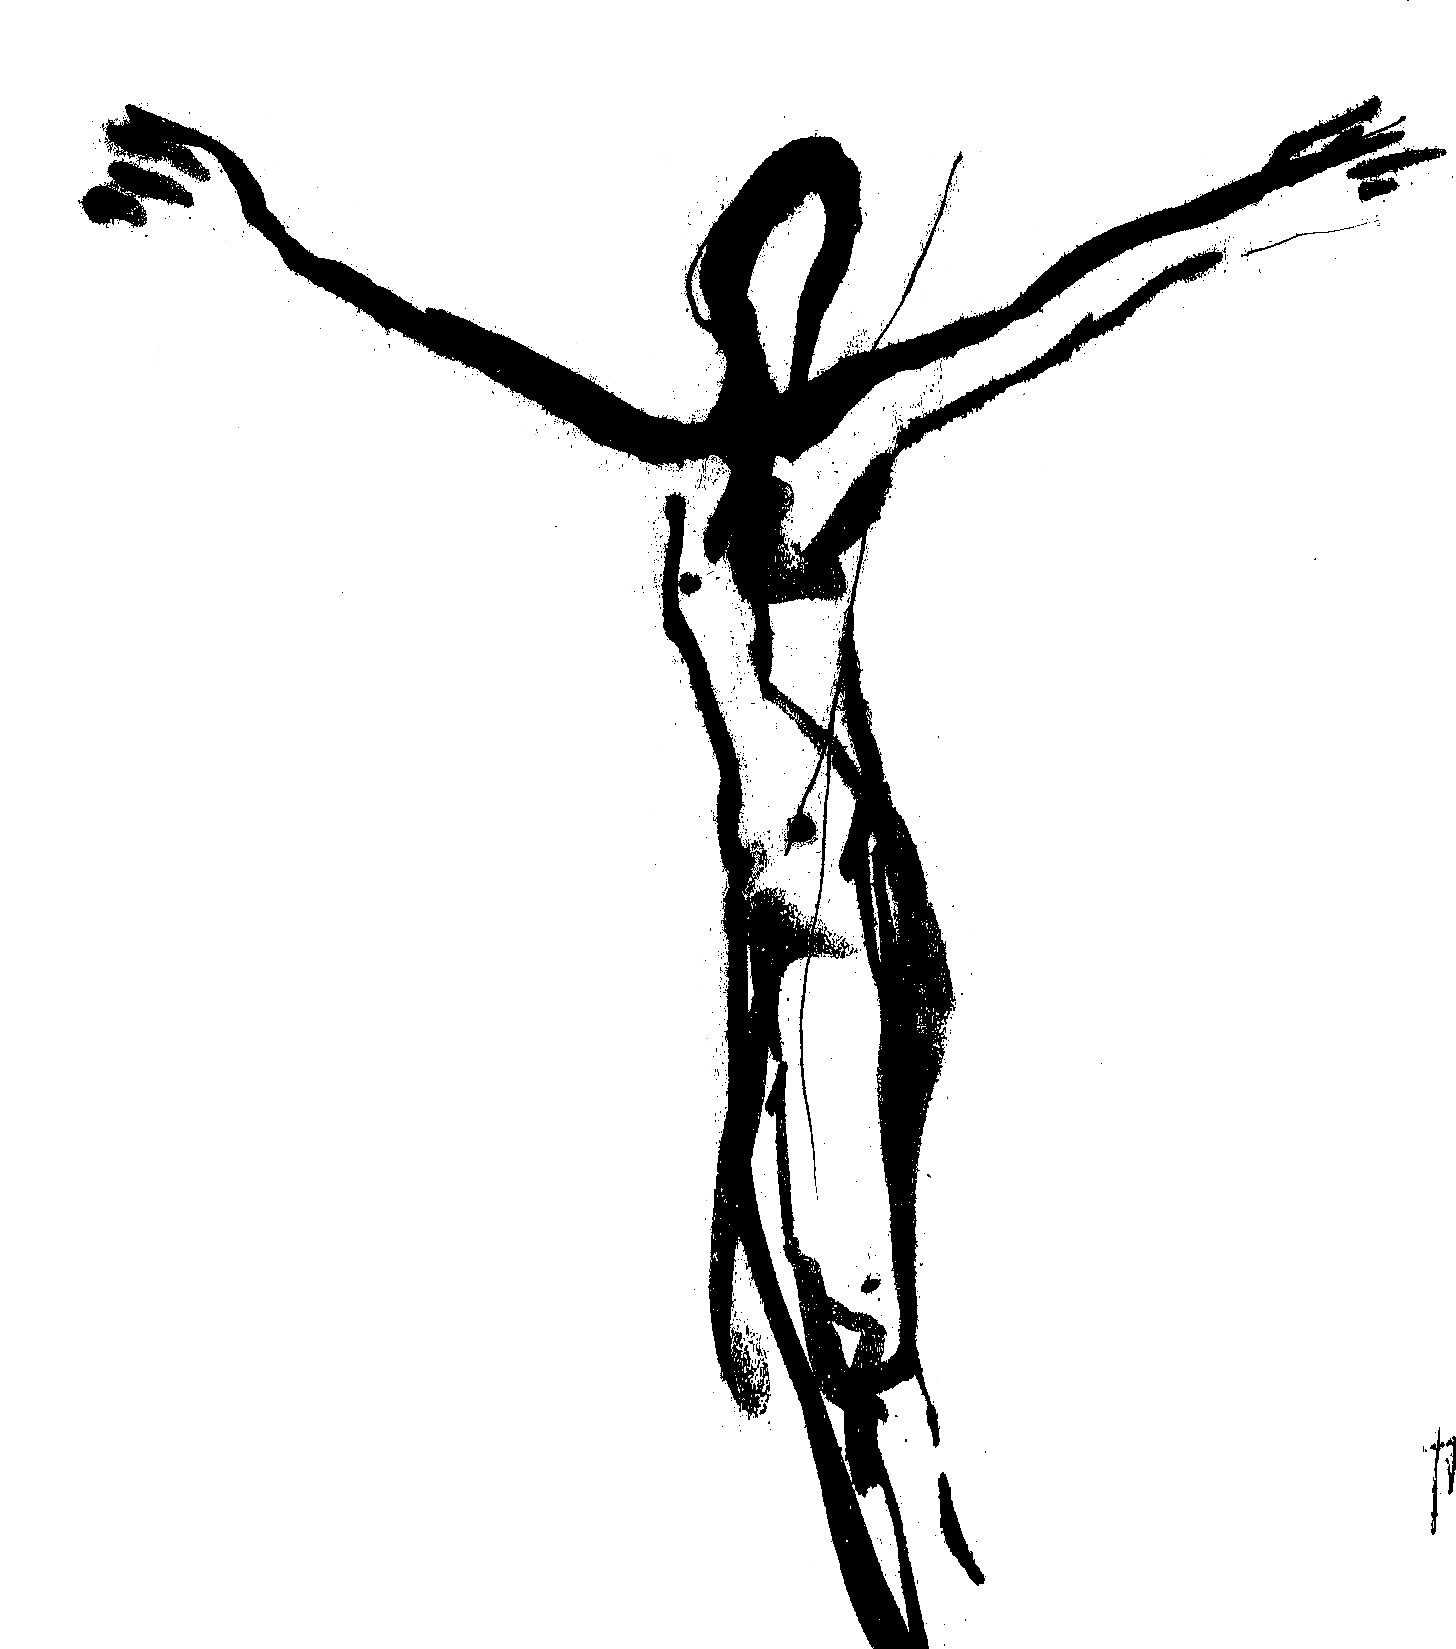
\includegraphics[height=8cm]{crux.jpg}
\end{center}

\vfill

\begin{center}
%Ad usum et secundum consuetudines chori \guillemotright{}Conventus Choralis\guillemotleft.

%Editio Sancti Wolfgangi \annusEditionis
\end{center}

\pagebreak

\renewcommand{\headrulewidth}{0pt} % no horiz. rule at the header
\fancyhf{}
\pagestyle{fancy}

\cantusSineNeumas

\pars{Oratio ante divinum Officium.}

\lettrine{{\color{red}A}}{peri,} Dómine, os meum ad benedicéndum nomen sanctum tuum:
munda quoque cor meum ab ómnibus vanis, pervérsis, et aliénis
cogitatiónibus:
intelléctum illúmina, afféctum inflámma,
ut digne, atténte ac devóte hoc Offícium recitáre váleam,
et exaudíri mérear ante conspéctum Divínæ Maiestátis tuæ.
Per Christum, Dóminum nostrum.
\Rbardot{} Amen.

Dómine, in unióne illíus divínæ intentiónis,
qua ipse in terris laudes Deo persolvísti,
has tibi Horas \rubricatum{(vel \textnormal{hanc tibi Horam})} persólvo.

%\trOratioAnteOfficium

\vfill

\pars{Oratio post divinum Officium.}

\rubrica{
  Orationem sequentem devote post Officium recitantibus
  Leo Papa X. defectus, et culpas in eo persolvendo ex humana
  fragilitate contractas, indulsit, et dicitur flexis genibus.
}

\lettrine{{\color{red}S}}{acrosánctæ} et indivíduæ Trinitáti,
crucifíxi Dómini nostri Iesu Christi humanitáti,
beatíssimæ et gloriosíssimæ sempérque Vírginis Maríæ
fecúndæ integritáti, 
et ómnium Sanctórum universitáti
sit sempitérna laus, honor, virtus et glória
ab omni creatúra,
nobísque remíssio ómnium peccatórum,
per infiníta sǽcula sæculórum.
\Rbardot{} Amen.

\noindent \Vbardot{} Beáta víscera Maríæ Virginis, quæ portavérunt
ætérni Patris Fílium.\\
\Rbardot{} Et beáta úbera, quæ lactavérunt Christum Dominum.

\rubrica{Et dicitur secreto \textnormal{Pater noster.} et \textnormal{Ave María.}}

%\trOratioPostOfficium

\vfill

\hora{Ad I. Vesperas.} %%%%%%%%%%%%%%%%%%%%%%%%%%%%%%%%%%%%%%%%%%%%%%%%%%%%%
%\sideThumbs{I. Vesperæ}

\vspace{5mm}
\grechangedim{interwordspacetext}{0.18 cm plus 0.15 cm minus 0.05 cm}{scalable}%
\cuminitiali{}{temporalia/deusinadiutorium-solemnis.gtex}
\grechangedim{interwordspacetext}{0.22 cm plus 0.15 cm minus 0.05 cm}{scalable}%

\vfill
\pagebreak

\pars{Psalmus 1.} \scriptura{\textbf{H257}}

\vspace{-4mm}

\antiphona{VII c}{temporalia/ant-omagnum.gtex}

%\trAntI

\scriptura{Ps. 112}

\initiumpsalmi{temporalia/ps112-initium-vii-c-auto.gtex}

%\psalmusEtTranslatioT{temporalia/ps112-comb.tex}{10cm}
\input{temporalia/ps112.tex} \Abardot{}

\vfill
\pagebreak

\pars{Psalmus 2.} \scriptura{\textbf{H257}}

\vspace{-4mm}

\antiphona{III a}{temporalia/ant-salvanos.gtex}

%\trAntII

\scriptura{Ps. 116}

\initiumpsalmi{temporalia/ps116-initium-iii-a-auto.gtex}
%\psalmusEtTranslatioT{temporalia/ps116-comb.tex}{10cm}
\input{temporalia/ps116.tex} \Abardot{}

\vfill
\pagebreak

\pars{Psalmus 3.} \scriptura{Cf. Ap. 5, 5; \textbf{H257}}

\vspace{-4mm}

\antiphona{I f}{temporalia/ant-eccecrucem.gtex}

%\trAntIII

\scriptura{Ps. 145}

\initiumpsalmi{temporalia/ps145-initium-i-f-auto.gtex}
%\psalmusEtTranslatioT{temporalia/ps145-comb.tex}{10cm}
\input{temporalia/ps145.tex} \Abardot{}

\vfill
\pagebreak

\pars{Psalmus 4.} \scriptura{Cf. Gal. 6, 14; \textbf{H258}}

\vspace{-4mm}

\antiphona{VII c}{temporalia/ant-nosautem.gtex}

%\trAntIV

\scriptura{Ps. 146}

\initiumpsalmi{temporalia/ps146-initium-vii-c-auto.gtex}
%\psalmusEtTranslatioT{temporalia/ps146-comb.tex}{10cm}
\input{temporalia/ps146.tex} \Abardot{}

\vfill
\pagebreak

\pars{Psalmus 5.} \scriptura{\textbf{H257}}

\vspace{-4mm}

\antiphona{II D}{temporalia/ant-persignumcrucis.gtex}

%\trAntIV

\scriptura{Ps. 147}

\initiumpsalmi{temporalia/ps147-initium-ii-D-auto.gtex}
%\psalmusEtTranslatioT{temporalia/ps147-comb.tex}{10cm}
\input{temporalia/ps147.tex} \Abardot{}

\vfill
\pagebreak

% Capitulum. %%%
\pars{Capitulum.} \scriptura{Philipp. 2, 5-7}

\cuminitiali{}{temporalia/capitulum-HocEnimSentite.gtex}

% preklad Jeruz. bible
%\trCapituli

\vfill
\pars{Responsorium.} \scriptura{\Vbardot{} Cf. Gal. 6, 14; \textbf{H256}}

\vspace{-5mm}

\responsorium{VII}{temporalia/resp-ocruxgloriosa-CROCHU.gtex}{}

%\trRespVesp

\vfill
\pagebreak

% Hymnus. %%%
\pars{Hymnus.} \scriptura{Venantius Fortunatus (sæc. VI); \textbf{C100}}

{
\grechangedim{interwordspacetext}{0.20 cm plus 0.15 cm minus 0.05 cm}{scalable}%
\cuminitiali{I}{temporalia/hym-CruxFidelis.gtex}
\grechangedim{interwordspacetext}{0.22 cm plus 0.15 cm minus 0.05 cm}{scalable}%
}
%\input{cantus/amon33/hym-CruxFidelis-bohtext.tex}

\vfill

\pars{Versus.}

% Versus. %%%
\sineinitiali{temporalia/versus-hocsignum.gtex}
    
\noindent %\trVersus

\vfill
\pagebreak

\pars{Canticum B. Mariæ V.} \scriptura{\textbf{H259}}

\vspace{-4mm}

\antiphona{I D\textsuperscript{2}}{temporalia/ant-ocruxsplendidior.gtex}

%\trAntMagnificatI

%\vspace{-3mm}

\scriptura{Lc. 1, 46-55}

%\vspace{-2mm}

\initiumpsalmi{temporalia/magnificat-initium-isoll-D2.gtex}

%\vspace{-1.5mm}

%\psalmusEtTranslatioT{temporalia/magnificat-comb.tex}{10.3cm}
\input{temporalia/magnificat.tex}

\vfill

\antiphona{}{temporalia/ant-ocruxsplendidior.gtex}

\vfill
\pagebreak

\anteOrationem

\pagebreak

%% Oratio. %%%
\pars{Oratio.}

\cuminitiali{}{temporalia/oratio.gtex}
%\trOrationis

\vfill

\rubrica{Hebdomadarius dicit iterum Dominus vobiscum, vel cantor dicit:}

\vspace{2mm}

\sineinitiali{temporalia/domineexaudi.gtex}

\rubrica{Postea cantatur a cantore:}

\vspace{2mm}

\cuminitiali{II}{temporalia/benedicamus-duplexmajus-vesperae.gtex}

\vspace{1mm}

\vfill
\pagebreak

\hora{Ad Matutinum.} %%%%%%%%%%%%%%%%%%%%%%%%%%%%%%%%%%%%%%%%%%%%%%%%%%%%%%%%%%
%\sideThumbs{Matutinum}

\vspace{2mm}

\cuminitiali{}{temporalia/dominelabiamea.gtex}

\vspace{2mm}

\pars{Invitatorium.}

\vspace{-2mm}

\antiphona{IV*}{temporalia/inv-christumregem.gtex}

\vfill
\pagebreak

\pars{Hymnus.}

\vspace{-5mm}

\antiphona{I}{temporalia/hym-SalveCruxSancta.gtex}

\vfill
\pagebreak

\subhora{In I. Nocturno}

\pars{Psalmus 1.} \scriptura{Lc. 24, 23.26; Gal. 3, 13}

\vspace{-4mm}

\antiphona{VI F}{temporalia/ant-crucifixussurrexit.gtex}

%\trMatAntI

\scriptura{Psalmus 1.}

\initiumpsalmi{temporalia/ps1-initium-vi-F-auto.gtex}

%\psalmusEtTranslatioT{temporalia/ps1-comb.tex}{10cm}
\input{temporalia/ps1.tex} \Abardot{}

%\antiphona{}{temporalia/ant-crucifixussurrexit.gtex} % repeat the antiphon - new page

\vfill
\pagebreak

\pars{Psalmus 2.} \scriptura{\textbf{H256}}

\vspace{-4mm}

\antiphona{I a\textsuperscript{2}}{temporalia/ant-ocruxadmirabilis.gtex}

%\trMatAntII

\scriptura{Psalmus 2.}

\initiumpsalmi{temporalia/ps2-initium-i-a2-auto.gtex}

%\psalmusEtTranslatioT{temporalia/ps2-comb.tex}{10cm}
\input{temporalia/ps2.tex} \Abardot{}

%\antiphona{}{temporalia/ant-ocruxadmirabilis.gtex} % repeat the antiphon - new page

\vfill
\pagebreak

\pars{Psalmus 3.} \scriptura{\textbf{H258}}

\vspace{-4mm}

\antiphona{VIII G}{temporalia/ant-tuamcrucemadoramus.gtex}

%\trMatAntIII

\scriptura{Psalmus 3.}

\initiumpsalmi{temporalia/ps3-initium-viii-G-auto.gtex}

%\psalmusEtTranslatioT{temporalia/ps3-comb.tex}{10cm}
\input{temporalia/ps3.tex} \Abardot{}

\vfill
\pagebreak

\pars{Versus.}

\sineinitiali{temporalia/versus-hocsignum.gtex}

\vspace{5mm}

\sineinitiali{temporalia/oratiodominica-mat.gtex}

\vspace{5mm}

\pars{Absolutio.}

\cuminitiali{}{temporalia/absolutio-exaudi.gtex}

%\trMatAbsolutioI

\vfill
\pagebreak

\cuminitiali{}{temporalia/benedictio-solemn-benedictione.gtex}

%\trMatBenedictioI

\vspace{7mm}

\pars{Lectio I.} \scriptura{Num. 21, 1-3}

\noindent De libro Númeri.

\noindent Cum audísset Chananǽus rex Arad, qui habitábat ad merídiem, venísse scílicet Israël per exploratórum viam, pugnávit contra illum et victor exsístens duxit ex eo prædam. At Israël, voto se Dómino óbligans, ait: Si tradíderis pópulum istum in manu mea, delébo urbes eius. Exaudivítque Dóminus preces Israël, et trádidit Chananǽum, quem ille interfécit, subvérsis úrbibus eius, et vocávit nomen loci illíus Horma, id est, anáthema.

\noindent \Vbardot{} Tu autem, Dómine, miserére nobis.
\noindent \Rbardot{} Deo grátias.

\vfill
\pagebreak

\iffalse
\pars{Responsorium 1.} \scriptura{\textbf{H305}}

\vspace{-5mm}

\responsorium{III}{temporalia/resp-hodienataest-CROCHU.gtex}{}
\fi

\vfill
\pagebreak

\cuminitiali{}{temporalia/benedictio-solemn-unigenitus.gtex}

%\trMatBenedictioII

\vspace{7mm}

\pars{Lectio II.} \scriptura{Num. 21, 4-6}

\noindent Profécti sunt autem et de monte Hor per viam quæ ducit ad Mare Rubrum, ut circumírent terram Edom. Et tædére cœpit pópulum itíneris ac labóris. Locutúsque contra Deum et Móysen ait: Cur eduxísti nos de Ægýpto ut morerémur in solitúdine? Deest panis, non sunt aquæ, ánima nostra iam náuseat super cibo isto levíssimo. Quam ob rem misit Dóminus in pópulum ignítos serpéntes.

\noindent \Vbardot{} Tu autem, Dómine, miserére nobis.
\noindent \Rbardot{} Deo grátias.

\vfill
\pagebreak

\iffalse
\pars{Responsorium 2.} \scriptura{\textbf{H305}}

\vspace{-5mm}

\responsorium{IV}{temporalia/resp-beatissimaevirginis-CROCHU.gtex}{}
\fi

\vfill
\pagebreak

\cuminitiali{}{temporalia/benedictio-solemn-spiritus.gtex}

%\trMatBenedictioIII

\vspace{7mm}

\pars{Lectio III.} \scriptura{Num. 21, 6-9}

\noindent Ad quorum plagas et mortes plurimórum venérunt ad Móysen atque dixérunt: Peccávimus, quia locúti sumus contra Dóminum et te: ora ut tollat a nobis serpéntes. Oravítque Móyses pro pópulo. Et locútus est Dóminus ad eum: Fac serpéntem ǽneum et pone eum pro signo: qui percússus aspéxerit eum, vivet. Fecit ergo Móyses serpéntem ǽneum et pósuit eum pro signo; quem cum percússi aspícerent, sanabántur.

\noindent \Vbardot{} Tu autem, Dómine, miserére nobis.
\noindent \Rbardot{} Deo grátias.

\vfill
\pagebreak

\iffalse
\pars{Responsorium 3.} \scriptura{\textbf{H305}}

\vspace{-5mm}

\responsorium{VII}{temporalia/resp-gloriosaevirginis-CROCHU.gtex}{}
\fi

\vfill
\pagebreak

\subhora{In II. Nocturno}

\pars{Psalmus 4.} \scriptura{\textbf{H356}}

\vspace{-4mm}

\antiphona{VIII G}{temporalia/ant-salvecruxquae.gtex}

%\trMatAntIV

\scriptura{Psalmus 4.}

\initiumpsalmi{temporalia/ps4-initium-viii-G-auto.gtex}

%\psalmusEtTranslatioT{temporalia/ps4-comb.tex}{10cm}
\input{temporalia/ps4.tex} \Abardot{}

%\antiphona{}{temporalia/ant-salvecruxquae.gtex} % repeat the antiphon - new page

\vfill
\pagebreak

\pars{Psalmus 5.} \scriptura{Phil. 1, 21; Gal. 6, 14; \textbf{H284}}

\vspace{-4mm}

\antiphona{I g}{temporalia/ant-mihivivere.gtex}

%\trMatAntV

\scriptura{Psalmus 10.}

\initiumpsalmi{temporalia/ps10-initium-i-g-auto.gtex}

%\psalmusEtTranslatioT{temporalia/ps10-comb.tex}{10cm}
\input{temporalia/ps10.tex} \Abardot{}

%\antiphona{}{temporalia/ant-mihivivere.gtex} % repeat the antiphon - new page

\vfill
\pagebreak

\pars{Psalmus 6.} \scriptura{\textbf{H259}}

\vspace{-4mm}

\antiphona{IV E}{temporalia/ant-adoremuscrucissignaculum.gtex}

%\trMatAntVI

\scriptura{Psalmus 20.}

\initiumpsalmi{temporalia/ps20-initium-iv-E-auto.gtex}

%\psalmusEtTranslatioT{temporalia/ps20-comb.tex}{10cm}
\input{temporalia/ps20.tex} \Abardot{}

%\antiphona{}{temporalia/ant-adoremuscrucissignaculum.gtex} % repeat the antiphon - new page

\vfill
\pagebreak

\pars{Versus.}

\sineinitiali{temporalia/versus-adoramuste.gtex}

\vspace{5mm}

\sineinitiali{temporalia/oratiodominica-mat.gtex}

\vspace{5mm}

\pars{Absolutio.}

\cuminitiali{}{temporalia/absolutio-ipsius.gtex}

%\trMatAbsolutioII

\vfill
\pagebreak

\cuminitiali{}{temporalia/benedictio-solemn-deus.gtex}

%\trMatBenedictioIV

\vspace{7mm}

\pars{Lectio IV.}

\noindent Chósroas, Persárum rex, extrémis Phocæ impérii tempóribus, Ægýpto et Africa occupáta ac Ierosólyma capta multísque ibi cæsis Christianórum míllibus, Christi Dómini Crucem, quam Hélena in monte Calváriæ collocárat, in Pérsidem ábstulit. Itaque Heraclíus, qui Phocæ succésserat, multis belli incómmodis et calamitátibus afféctus, pacem petébat; quam a Chósroa, victóriis insolénte, ne iníquis quidem conditiónibus impetráre póterat. Quare in summo discrímine se assíduis ieiúniis et oratiónibus exércens, opem a Deo veheménter implorábat; cuius mónitu exércitu comparáto, signa cum hoste cóntulit, ac tres duces Chósroæ cum tribus exercítibus superávit.

\noindent \Vbardot{} Tu autem, Dómine, miserére nobis.
\noindent \Rbardot{} Deo grátias.

\vfill
\pagebreak

\iffalse
\pars{Responsorium 4.} \scriptura{\textbf{H306}}

\vspace{-5mm}

\responsorium{I}{temporalia/resp-nativitasgloriosae-CROCHU.gtex}{}
\fi

\vfill
\pagebreak

\cuminitiali{}{temporalia/benedictio-solemn-christus.gtex}

%\trMatBenedictioV

\vspace{7mm}

\pars{Lectio V.}

\noindent Quibus cládibus fractus Chósroas, in fuga, qua traícere Tigrim parábat, Medársen fílium sócium regni desígnat. Sed eam contuméliam cum Síroës, Chósroæ maior natu fílius, ferret atróciter, patri simul et fratri necem machinátur; quam paulo post utríque ex fuga retrácto áttulit, regnúmque ab Heraclío impetrávit quibúsdam accéptis conditiónibus, quarum ea prima fuit, ut Crucem Christi Dómini restitúeret. Ergo Crux, quatuórdecim annis postquam vénerat in potestátem Persárum, recépta est. Quam rédiens Ierosólymam Heraclíus solémni celebritáte suis húmeris rétulit in eum montem, quo eam Salvátor túlerat.

\noindent \Vbardot{} Tu autem, Dómine, miserére nobis.
\noindent \Rbardot{} Deo grátias.

\vfill
\pagebreak

\iffalse
\pars{Responsorium 5.}

\vspace{-5mm}

\responsorium{VIII}{temporalia/matresp5.gtex}{}
\fi

\vfill
\pagebreak

\cuminitiali{}{temporalia/benedictio-solemn-ignem.gtex}

%\trMatBenedictioVI

\vspace{7mm}

\pars{Lectio VI.}

\noindent Quod factum illústri miráculo commendátum est. Nam Heraclíus, ut erat auro et gemmis ornátus, insístere coáctus est in porta, quæ ad Calváriæ montem ducébat. Quo enim magis prógredi conabátur, eo magis retinéri videbátur. Cumque ea re et ipse Heraclíus et réliqui omnes obstupéscerent; Zacharías, Ierosolymórum antístes, Vide, inquit, imperátor, ne isto triumpháli ornátu, in Cruce ferénda parum Iesu Christi paupertátem et humilitátem imitére. Tum Heraclíus, abiécto amplíssimo vestítu detractísque cálceis ac plebéio amíctu indútus, réliquum viæ fácile confécit, et in eódem Calváriæ loco Crucem státuit, unde fúerat a Persis asportáta. Itaque Exaltatiónis sanctæ Crucis solémnitas, quæ hac die quotánnis celebrabátur, illústrior habéri cœpit ob eius rei memóriam, quod ibídem fúerit repósita ab Heraclío, ubi Salvatóri primum fúerat constitúta.

\noindent \Vbardot{} Tu autem, Dómine, miserére nobis.
\noindent \Rbardot{} Deo grátias.

\vfill
\pagebreak

\iffalse
\pars{Responsorium 6.} \scriptura{\Rbardot{} Cantor \Vbardot{} Lc. 1, 42; \textbf{H307}}

\vspace{-5mm}

\responsorium{I}{temporalia/resp-nativitastua-CROCHU.gtex}{}
\fi

\vfill
\pagebreak

\subhora{In III. Nocturno}

\pars{Psalmus 7.}

\vspace{-4mm}

\antiphona{VIII G}{temporalia/ant-propterlignum.gtex}

%\vspace{-4mm}

%\trMatAntVII

\scriptura{Psalmus 95.}

\initiumpsalmi{temporalia/ps95-initium-viii-G-auto.gtex}

%\psalmusEtTranslatioT{temporalia/ps95-comb.tex}{10.5cm}
\input{temporalia/ps95.tex}

\vfill

\antiphona{}{temporalia/ant-propterlignum.gtex} % repeat the antiphon - new page

\vfill
\pagebreak

\pars{Psalmus 8.} \scriptura{\textbf{H258}}

\antiphona{VII a}{temporalia/ant-salvatormundi.gtex}

%\trMatAntVIII

\scriptura{Psalmus 96.}

\initiumpsalmi{temporalia/ps96-initium-vii-a-auto.gtex}

%\psalmusEtTranslatioT{temporalia/ps96-comb.tex}{10cm}
\input{temporalia/ps96.tex}

\vfill

\antiphona{}{temporalia/ant-salvatormundi.gtex} % repeat the antiphon - new page

\vfill
\pagebreak

\pars{Psalmus 9.} \scriptura{\textbf{H258}}

\antiphona{I g}{temporalia/ant-adoramustechriste.gtex}

%\trMatAntIX

\scriptura{Psalmus 97.}

\initiumpsalmi{temporalia/ps97-initium-i-g-auto.gtex}

%\psalmusEtTranslatioT{temporalia/ps97-comb.tex}{10cm}
\input{temporalia/ps97.tex} \Abardot{}

\vfill
\pagebreak

\pars{Versus.}

\sineinitiali{temporalia/versus-omnisterra.gtex}

\vspace{5mm}

\sineinitiali{temporalia/oratiodominica-mat.gtex}

\vspace{5mm}

\pars{Absolutio.}

\cuminitiali{}{temporalia/absolutio-avinculis.gtex}

%\trMatAbsolutioIII

\vfill
\pagebreak

\cuminitiali{}{temporalia/benedictio-solemn-evangelica.gtex}

%\trMatBenedictioVII

\vspace{7mm}

\pars{Lectio VII.} \scriptura{Io. 12, 31-36}

\noindent Léctio sancti Evangélii secúndum Ioánnem.

\noindent In illo témpore: Dixit Iesus turbis Iudæórum: Nunc iudícium est mundi, nunc princeps huius mundi eiciétur foras. Et réliqua.

\scriptura{Sermo 8 de Passione Domini, post medium}

\noindent Homilía sancti Leónis Papæ.

\noindent Exaltáto, dilectíssimi, per Crucem Christo, non illa tantum spécies aspéctui mentis occúrrat, quæ fuit in óculis impiórum, quibus per Móysen dictum est: Et erit pendens vita tua ante óculos tuos, et timébis die ac nocte, et non credes vitæ tuæ. Isti enim nihil in crucifíxo Dómino præter fácinus suum cogitáre potuérunt, habéntes timórem, non quo fides vera iustificátur, sed quo consciéntia iníqua torquétur. Noster vero intelléctus, quem spíritus veritátis illúminat, glóriam Crucis, cælo terráque radiántem, puro ac líbero corde suscípiat; et interióre ácie vídeat, quale sit quod Dóminus, cum de passiónis suæ loquerétur instántia, dixit: Nunc iudícium mundi est, nunc princeps huius mundi eiciétur foras. Et ego, si exaltátus fúero a terra, ómnia traham ad meípsum.

\noindent \Vbardot{} Tu autem, Dómine, miserére nobis.
\noindent \Rbardot{} Deo grátias.

\vfill
\pagebreak

\iffalse
\pars{Responsorium 7.} \scriptura{\Rbardot{} Lc. 1, 48 \Vbardot{} ibid. 1, 50; \textbf{H297}}

\vspace{-5mm}

\responsorium{VIII}{temporalia/resp-beatammedicent-CROCHU.gtex}{}
\fi

\vfill
\pagebreak

\cuminitiali{}{temporalia/benedictio-solemn-divinum.gtex}

%\trMatBenedictioVIII

\vspace{7mm}

\pars{Lectio VIII.}

\noindent O admirábilis poténtia Crucis! o ineffábilis glória Passiónis, in qua et tribúnal Dómini, et iudícium mundi, et potéstas est Crucifíxi! Traxísti enim, Dómine, ómnia ad te, et cum expandísses tota die manus tuas ad pópulum non credéntem et contradicéntem, tibi, confiténdæ maiestátis tuæ sensum totus mundus accépit. Traxísti, Dómine, ómnia ad te, cum in exsecratiónem Iudáici scéleris, unam protulérunt ómnia eleménta senténtiam; cum, obscurátis lumináribus cæli et convérso in noctem die, terra quoque mótibus quaterétur insólitis, univérsaque creatúra impiórum úsui se negáret. Traxísti, Dómine, ómnia ad te, quóniam, scisso templi velo, Sancta sanctórum ab indígnis pontifícibus recessérunt; ut figúra in veritátem, prophetía in manifestatiónem, et lex in Evangélium verterétur.

\noindent \Vbardot{} Tu autem, Dómine, miserére nobis.
\noindent \Rbardot{} Deo grátias.

\vfill
\pagebreak

\pars{Responsorium 8.} \scriptura{\Vbardot{} Cf. Gal. 6, 14; \textbf{H256}}

\vspace{-5mm}

\responsorium{VII}{temporalia/resp-ocruxgloriosa-CROCHU.gtex}{}

\vfill
\pagebreak

\cuminitiali{}{temporalia/benedictio-solemn-adsocietatem.gtex}

%\trMatBenedictioIX

\vspace{7mm}

\pars{Lectio IX.}

\noindent Traxísti, Dómine, ómnia ad te, ut, quod in uno Iudǽæ templo obumbrátis significatiónibus tegebátur, pleno apertóque sacraménto universárum ubíque natiónum devótio celebráret. Nunc étenim et ordo clárior levitárum, et dígnitas ámplior seniórum, et sacrátior est únctio sacerdótum: quia Crux tua ómnium fons benedictiónum, ómnium est causa gratiárum; per quam credéntibus datur virtus de infirmitáte, glória de oppróbrio, vita de morte. Nunc étiam, carnálium sacrificiórum varietáte cessánte, omnes differéntias hostiárum una córporis et sánguinis tui implet oblátio: quóniam tu es verus Agnus Dei, qui tollis peccáta mundi; et ita in te univérsa pérficis mystéria, ut sicut unum est pro omni víctima sacrifícium, ita unum de omni gente sit regnum.

\noindent \Vbardot{} Tu autem, Dómine, miserére nobis.
\noindent \Rbardot{} Deo grátias.

\vfill
\pagebreak

% Te Deum

\pars{Hymnus Ambrosianus} \scriptura{Tonus Solemnis}

\vspace{-2mm}

{
\grechangedim{interwordspacetext}{0.26 cm plus 0.15 cm minus 0.05 cm}{scalable}%
\cuminitiali{III}{temporalia/tedeum-solemnis-gn.gtex}
\grechangedim{interwordspacetext}{0.22 cm plus 0.15 cm minus 0.05 cm}{scalable}%
}

%\trTeDeum

\vfill
\pagebreak

\sineinitiali{temporalia/domineexaudi.gtex}

\vfill

\pars{Oratio.}

\cuminitiali{}{temporalia/oratio.gtex}
%\trOrationis

\vfill

\noindent \Vbardot{} Dómine, exáudi oratiónem meam.
\Rbardot{} Et clamor meus ad te véniat.

\vfill

% Nocturnale Romanum 2002, p. LXXVI Benedicamus Domino seems to match
% the one from Solemn Laudes.
\cuminitiali{V}{temporalia/benedicamus-solemnis-laud.gtex}

\vfill

\noindent \Vbardot{} Fidélium ánimæ per misericórdiam Dei requiéscant in pace.
\Rbardot{} Amen.

%\trFideliumAnimae

\vfill
\pagebreak

\iffalse
\hora{Ad Laudes.} %%%%%%%%%%%%%%%%%%%%%%%%%%%%%%%%%%%%%%%%%%%%%%%%%%%%%%%%%%
%\sideThumbs{Laudes}

% Psalmi festivi (AM33, pg. 721):
% 66 // 92, 99, 62, Dan3, 148+149+150

\vspace{1cm}
\cuminitiali{}{temporalia/deusinadiutorium-alter.gtex}
\vspace{1cm}

\cantusSineNeumas

\pars{Psalmus 1.} \scriptura{Ps. 66}

\initiumpsalmi{temporalia/ps66-initium-dir-auto.gtex}

%\psalmusEtTranslatioT{temporalia/ps66-comb.tex}{10cm}
\input{temporalia/ps66.tex} \Abardot{}

\vfill
\pagebreak

\pars{Psalmus 2.} \scriptura{\textbf{H307}}

\antiphona{VIII G}{temporalia/ant-nativitasgloriosae.gtex}

%\trAntI

\scriptura{Ps. 92}

\initiumpsalmi{temporalia/ps92-initium-viii-G-auto.gtex}

%\psalmusEtTranslatioT{temporalia/ps92-comb.tex}{10cm}
\input{temporalia/ps92.tex} \Abardot{}

\vfill
\pagebreak

\pars{Psalmus 3.} \scriptura{\textbf{H307}}

\antiphona{VII c}{temporalia/ant2.gtex}

%\trAntII

\scriptura{Ps. 99}

\initiumpsalmi{temporalia/ps99-initium-vii-c-auto.gtex}

%\psalmusEtTranslatioT{temporalia/ps99-comb.tex}{10cm}
\input{temporalia/ps99.tex} \Abardot{}

\vfill
\pagebreak

\pars{Psalmus 4.} \scriptura{\textbf{H307}}

\vspace{-4mm}

\antiphona{VI C}{temporalia/ant-regaliexprogenie.gtex}

\vspace{-2mm}

%\trAntIII

\scriptura{Ps. 62.}

\initiumpsalmi{temporalia/ps62-initium-vi-C.gtex}

%\vspace{-6mm}

%\psalmusEtTranslatioT{temporalia/ps62-comb.tex}{10cm}
\input{temporalia/ps62.tex} \Abardot{}

\vfill
\pagebreak

\pars{Psalmus 5.} \scriptura{\textbf{H308}}

\vspace{-4mm}

\antiphona{VIII G}{temporalia/ant-cordeetanimo.gtex}

\vspace{-2mm}

%\trAntIV

\scriptura{Canticum trium puerorum, Dan. 3, 57-88 et 56}

\vspace{-2mm}

\initiumpsalmi{temporalia/dan3-initium-viii-G-auto.gtex}

%\psalmusEtTranslatioT{temporalia/dan3-comb.tex}{10cm}
\input{temporalia/dan3.tex}

\rubrica{Hic non dicitur Gloria Patri, neque Amen.}
\vspace{1cm}

\antiphona{}{temporalia/ant-cordeetanimo.gtex} % repeat the antiphon - new page

\vfill
\pagebreak

\pars{Psalmus 6.} \scriptura{\textbf{H308}}

\vspace{-6mm}

\antiphona{VII c}{temporalia/ant5.gtex}

\vspace{-4mm}

%\trAntV

\scriptura{Ps. 148}

\vspace{-2mm}

\initiumpsalmi{temporalia/ps148-initium-vii-c-auto.gtex}

\vspace{-1.5mm}

%\psalmusEtTranslatioT{temporalia/ps148-comb.tex}{10cm}
\input{temporalia/ps148.tex} \rubrica{Hic non dicitur Gloria Patri.}

\vspace{-5mm}

\vfill
\pagebreak

%
\scriptura{Ps. 149}

\initiumpsalmi{temporalia/ps149-initium-vii-c-auto.gtex}

%\psalmusEtTranslatioT{temporalia/ps149-comb.tex}{10cm}
\input{temporalia/ps149.tex}

\rubrica{Hic non dicitur Gloria Patri.}

\vfill
\pagebreak

%
\scriptura{Ps. 150}

\initiumpsalmi{temporalia/ps150-initium-vii-c-auto.gtex}

%\psalmusEtTranslatioT{temporalia/ps150-comb.tex}{10cm}
\input{temporalia/ps150.tex}

\antiphona{}{temporalia/ant5.gtex} % repeat the antiphon - new page

\vfill
\pagebreak

\cantusSineNeumas

\pars{Capitulum.} \scriptura{Sir. 24, 14}

\cuminitiali{}{temporalia/capitulum-AbInitio.gtex}

% preklad Jeruz. bible
%\trCapituli

\vfill
\pars{Responsorium breve.}

\antiphona{VI}{temporalia/resp1v.gtex}

%\trRespVesp

\vfill
\pagebreak

\pars{Hymnus.}

\cuminitiali{II}{temporalia/hym-OSanctaMundiDomina.gtex}
%\input{cantus/amon33/hym-OSanctaMundiDomina-bohtext.tex}

\vfill

\pars{Versus.}

% Versus. %%%
\sineinitiali{temporalia/versus-nativitasest.gtex}
    
\noindent %\trVersus

\vfill
\pagebreak

\pars{Canticum Zachariæ.} \scriptura{\textbf{H308}}

\antiphona{VIII G}{temporalia/ant-nativitatemhodiernam.gtex}

%\trAntBenedictus

\scriptura{Lc. 1, 68-79}

\initiumpsalmi{temporalia/benedictus-initium-viiisoll-G-auto.gtex}

%\psalmusEtTranslatioT{temporalia/benedictus-comb.tex}{10cm}
\input{temporalia/benedictus.tex}

\antiphona{}{temporalia/ant-nativitatemhodiernam.gtex} % repeat the antiphon - new page

\vfill
\pagebreak

\cantusSineNeumas

\anteOrationem

\pagebreak

% Oratio. %%%
\pars{Oratio.}

\cuminitiali{}{temporalia/oratio.gtex}
%\trOrationis

\vfill

\rubrica{Hebdomadarius dicit iterum Dominus vobiscum, vel cantor dicit:}

\vspace{2mm}

\sineinitiali{temporalia/domineexaudi.gtex}

\rubrica{Postea cantatur a cantore:}

\vspace{2mm}

\cuminitiali{VIII}{temporalia/benedicamus-duplexmajus-laudes.gtex}

\vspace{1mm}

\vfill
\pagebreak

\hora{Ad II. Vesperas.} %%%%%%%%%%%%%%%%%%%%%%%%%%%%%%%%%%%%%%%%%%%%%%%%%%%%%
%\sideThumbs{I. Vesperæ}

%\vspace{5mm}
\grechangedim{interwordspacetext}{0.18 cm plus 0.15 cm minus 0.05 cm}{scalable}%
\cuminitiali{}{temporalia/deusinadiutorium-solemnis.gtex}
\grechangedim{interwordspacetext}{0.22 cm plus 0.15 cm minus 0.05 cm}{scalable}%

%\vfill
%\pagebreak

\pars{Psalmus 1.} \scriptura{\textbf{H307}}

\vspace{-4mm}

\antiphona{VIII G}{temporalia/ant-nativitasgloriosae.gtex}

\vspace{-2mm}

%\trAntI

\scriptura{Ps. 109}

\initiumpsalmi{temporalia/ps109-initium-viii-G-auto.gtex}

%\psalmusEtTranslatioT{temporalia/ps109-comb.tex}{10cm}
\input{temporalia/ps109.tex} \Abardot{}

\vfill
\pagebreak

\pars{Psalmus 2.} \scriptura{\textbf{H307}}

\antiphona{VII c}{temporalia/ant2.gtex}

%\trAntII

\scriptura{Ps. 112}

\initiumpsalmi{temporalia/ps112-initium-vii-c-auto.gtex}
%\psalmusEtTranslatioT{temporalia/ps112-comb.tex}{10cm}
\input{temporalia/ps112.tex} \Abardot{}

\vfill
\pagebreak

\pars{Psalmus 3.} \scriptura{\textbf{H307}}

\antiphona{VI C}{temporalia/ant-regaliexprogenie.gtex}

%\trAntIII

\scriptura{Ps. 121}

\initiumpsalmi{temporalia/ps121-initium-vi-C.gtex}
%\psalmusEtTranslatioT{temporalia/ps121-comb.tex}{10cm}
\input{temporalia/ps121.tex} \Abardot{}

\vfill
\pagebreak

\pars{Psalmus 4.} \scriptura{\textbf{H308}}

\antiphona{VIII G}{temporalia/ant-cordeetanimo.gtex}

%\trAntIV

\scriptura{Ps. 126}

\initiumpsalmi{temporalia/ps126-initium-viii-G-auto.gtex}
%\psalmusEtTranslatioT{temporalia/ps126-comb.tex}{10cm}
\input{temporalia/ps126.tex} \Abardot{}

\vfill
\pagebreak

% Capitulum. %%%
\pars{Capitulum.} \scriptura{Sir. 24, 14}

\cuminitiali{}{temporalia/capitulum-AbInitio.gtex}

% preklad Jeruz. bible
%\trCapituli

\vfill
\pars{Responsorium breve.}

\antiphona{VI}{temporalia/resp1v.gtex}

%\trRespVesp

\vfill
\pagebreak

% Hymnus. %%%
\pars{Hymnus.}

{
\grechangedim{interwordspacetext}{0.20 cm plus 0.15 cm minus 0.05 cm}{scalable}%
\cuminitiali{IV}{temporalia/hym-AveMarisStella-iv.gtex}
\grechangedim{interwordspacetext}{0.22 cm plus 0.15 cm minus 0.05 cm}{scalable}%
}
%\begin{translatioMulticol}{3}
Zdrávas, hvězdo mořská, životodárná Matko Boží\\
a vždy Panno, šťastná nebes bráno.\\
\\
Přijímajíc ono Ave z Gabrielových úst,\\
upevni nás v pokoji, měníc jméno Evy.\\
\textit{(Slovní hříčka Ave - Eva.)}\columnbreak

Rozvaž pouta vinným, dej světlo slepým:\\
odežeň, co je na nás špatného, vypros všechno dobré.\\
\\
Ukaž, že jsi matka: skrze tebe ať přijme (naše) prosby\\
ten, jenž, když se pro nás narodil, přijal i to, že bude tvůj.\\
\\
Jedinečná Panno, mezi všemi mírná,\\
zbav nás našich hříchů, učiň mírnými a čistými.\columnbreak

Dej nám čistý život, připrav nám svou cestu:\\
abychom viděli Ježíše a vždy se s tebou radovali.\\
\\
Buď chvála Bohu Otci, nejvyššímu Kristu důs\-toj\-nost,\\
(tak i) Duchu Svatému; Třem jediná pocta.\\
Amen.
\end{translatioMulticol}


\vfill

\pars{Versus.}

% Versus. %%%
\sineinitiali{temporalia/versus-nativitasest.gtex}
    
\noindent %\trVersus

\vfill
\pagebreak

\pars{Canticum B. Mariæ V.} \scriptura{\textbf{H308}}

\antiphona{I f}{temporalia/ant-nativitastua.gtex}

%\trAntMagnificatII

\scriptura{Lc. 1, 46-55}

\initiumpsalmi{temporalia/magnificat-initium-isoll-f.gtex}

%\psalmusEtTranslatioT{temporalia/magnificat-comb.tex}{10.3cm}
\input{temporalia/magnificat.tex}

\antiphona{}{temporalia/ant-nativitastua.gtex}

\vfill
\pagebreak

\anteOrationem

\pagebreak

%% Oratio. %%%
\pars{Oratio.}

\cuminitiali{}{temporalia/oratio.gtex}
%\trOrationis

\vfill

\rubrica{Hebdomadarius dicit iterum Dominus vobiscum, vel cantor dicit:}

\vspace{2mm}

\sineinitiali{temporalia/domineexaudi.gtex}

\rubrica{Postea cantatur a cantore:}

\vspace{2mm}

\cuminitiali{II}{temporalia/benedicamus-duplexmajus-vesperae.gtex}

\vspace{1mm}

\vfill
\pagebreak
\fi

\end{document}
